\section{Background}
\label{section:background}

\subsection{Passivity}
 
Passivity is a property of physical systems, defined as a constraint that the output energy 
is bounded by the input energy so far as well as any stored energy.  In control system design,
passive components are themselves stable, and interconnected passive systems are compositional 
with respect to stability (subject to a few constraints on the interconnections).  Frequently 
controllers are designed to be passive in order to gain this property.  Digital controller 
designs can also be passive, and are insensitive to many kinds of errors introduced when the
digital design is deployed to a computer platform. Platform behavior effects such as data and 
parameter quantization \cite{pass:fettweis86} and timing delays due to processor scheduling and 
network communications \cite{ncs:chopra} \cite{ncs:kottenstette07} have little effect on the
stability of a passive control design.  

Passivity guarantees bounded-input/bounded-output (BIBO) stability, and with a few additional 
constraints can also ensure asymptotic stability, which is  necessary for tracking. De la Sen
\cite{pass:delasen2} develops the concept of passivity formally using the following discussion.  
Let $u(t)$, $y(t)$, $D(t)$, and $S(t)$ be real-valued time-domain functions representing 
respectively, the input signals, output signals, dissipated energy, and stored energy.  
Then the power balance for a system is given by 

\begin{equation}
 u(t)y(t) = \dot{S}(t) + \dot{D}(t)
\end{equation}

and the energy balance is given as

\begin{equation}
 \left \langle u,y \right \rangle_t = S(t) + D(t) - S(0) - D(0).
\end{equation}

The dot superscript denotes the time-derivative, and the inner product is
the $L_2$ inner product of the two signals.  Then using this notation, the component
is passive if $\dot{D}(t) \geq 0$.  Then $D(t) \geq D(0)$, $u(t)y(t) \geq \dot{S}(t)$, 
and 

\begin{equation}
 \left \langle u,y \right \rangle_t \geq S(t) - S(0).
\end{equation}

Intuitively, the output can not exceed the sum of input energy and any remaining stored energy.
As far as interconnections, parallel and feedback interconnections of control components maintain
passivity, but serial interconnections may not.

\subsection{Towards a Sufficient Stability Condition}

Most approaches to nonlinear control system design rely on continuous time assumptions.  When we 
consider discrete time implementation in software subject to network delays and finite-precision 
quantization effects, linear approximations and high sample rates tend to be used to obtain 
tractable analysis and realizable execution.  In practice we have found that compositional techniques 
based on passivity have allowed us to construct reasonably low data rate digital controllers for 
nonlinear systems without resorting to conservative linear approximations. 

Passive control techniques have proven successful for many cases of nonlinear continuous time 
controllers, but nonlinear discrete time control poses several challenges.  Unfortunately many 
control structures are not passive in discrete time.  If we can approximate our controlled system 
as a cascade of passive systems then we can apply a systematic control design strategy, for 
which stability can be validated online.  After presenting the relevant
theory we will illustrate our control design approach using a simple example.

\subsection{Nonlinear Sector Analysis}

Digital control for nonlinear physical systems with fast dynamics (such as a quadrotor helicopter) 
use a zero-order hold to convert control values produced at discrete time instants into step 
functions held over a continuous interval of time.  For certain inputs and state trajectories, the 
hold process can introduce small amounts of new energy into the environment, violating passivity.  
The sector bounds analysis proposed by Zames \cite{control:sectors1} can be used to assess the 
amount of ``active'' (energy-producing) behavior which we can expect from a design under nominal 
operating conditions.

\begin{figure}[htb]
\centering
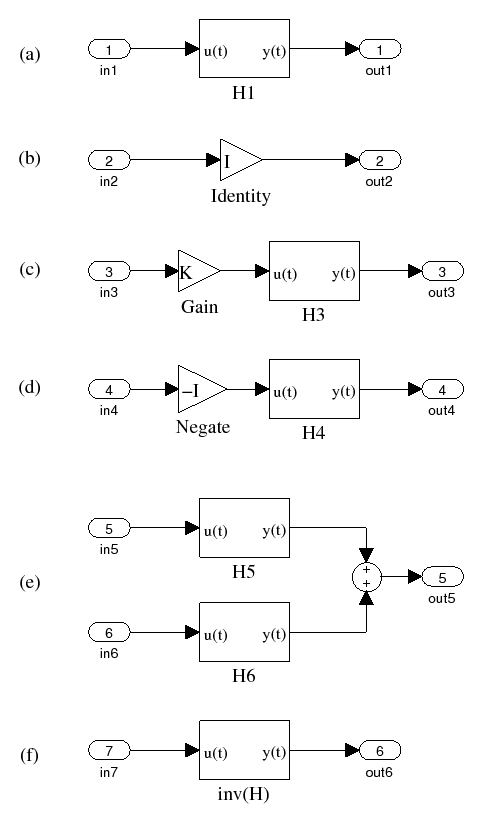
\includegraphics[width=0.95\columnwidth]{figures/mod_examples.png}
    \caption{Block diagram interconnection examples for conic system composition rules.}
    \label{fig:examples}
\end{figure}

Zames critical insight was that many causal nonlinear systems' dynamic input-output relationships 
can be confined to being either inside or outside a conic region. Systems whose input-output 
relationships can be confined inside a conic region are known as interior conic systems. Equivalently 
these interior conic systems can be described as residing {\em inside the sector} $[a,b]$ in 
which $a$ and $b$ are
real coefficients\cite{control:sectors1}. If there exist a real coefficients $a$ and $b$ such that 
Eq. \ref{eq:sectors} is satisfied then the system is an interior conic system inside the sector 
$[a,b]$ conversely if the inequality of Eq. \ref{eq:sectors} is reversed the system is exterior 
conic and outside the sector $[a,b]$. Table \ref{tab:quantities} describes the quantities
used in Eq. 4. For the special case when $|a| < b < \infty$, $b$ is also the gain of the system 
(i.e. $\lVert y_T \rVert_2 \leq b \lVert u_T \rVert_2$). For linear time invariant (LTI) single input single 
output (SISO) systems the term $a$ is the most negative real part of its corresponding Nyquist 
plot, it therefore is an approximate measure of the phase shift of a stable system. A passive 
system is equivalent to an interior conic system which is inside the sector $[0,\infty]$ 
therefore a passive LTI SISO system has no more than +/-90 degrees of phase shift in which all 
real parts of its corresponding Nyquist plot are {\em positive real}.

\begin{equation} 
\lVert y_T \rVert^2_2 - (a+b) \langle y,u \rangle_T + ab \lVert u_T \rVert^2_2 \leq 0
\label{eq:sectors}
\end{equation}

\begin{table}[htb]
\centering
\begin{tabular}[width=0.9\columnwidth]{@{\extracolsep{\fill}}  | c | l | }
\hline
\textbf{Quantity} & \textbf{Description} \\
\hline \hline
$u(t)$ & Input signal \\
\hline
$y(t)$ & Output signal \\
\hline
 & Energy produced by the component so far \\
$\lVert y_T \rVert^2_2$ & (output) in a time interval of length $T$. \\
\hline
 & Energy received by the component so far \\
$\lVert u_T \rVert^2_2$ & (input) in a time interval of length $T$. \\
\hline
 & Correlation between the input and output \\ 
$\langle y,u \rangle_T$ & sample values in a time interval of length $T$. \\
 & This is a measure of dissipation. \\
\hline
$a$ & Real-valued lower bound for the sector. \\
\hline
$b$ & Real-valued upper bound for the sector. \\
\hline
\end{tabular}
\caption{ Quantities for the sector formula.}
\label{tab:quantities}
\end{table}

A conic system can also be modeled as a functional relation between the possible input and output
signal spaces.  This corresponds intuitively to a causal block diagram where the function
specified in the block relates the inputs to the outputs, as in Fig. \ref{fig:examples} (a). 
See Zames for a complete formal functional description of sector analysis.
Given conic relations $H, H_1$ with $H$ in $[a,b]$ and $H_1$ in $[a_1, b_1]$ ($b, b_1 > 0$),
and given a constant $k \geq 0$,  we have the following sector composition rules from 
\cite{control:sectors1}:

\begin{enumerate}
\item $I$ is in $[1,1]$ (Fig. \ref{fig:examples} (b))
\item $kH$ is in $[ka, kb]$ (Fig. \ref{fig:examples} (c))
\item $-H$ is in $[-b, -a]$ (Fig. \ref{fig:examples} (d))
\item sum rule $H+H_1$ is in $[a+a_1, b+b_1]$ (Fig. \ref{fig:examples} (e))
\item inverse rule(s) (Fig. \ref{fig:examples} (f))
\begin{enumerate}
 \item $a > 0 \rightarrow H^{-1}$ is in $[\frac{1}{b},\frac{1}{a}]$.
 \item $a < 0 \rightarrow H^{-1}$ is outside $[\frac{1}{a},\frac{1}{b}]$.
 \item $a = 0 \rightarrow (H^{-1} - (\frac{1}{b}I)$ is positive.
\end{enumerate}
\end{enumerate}

For rule 5 an inverse system model must be well-defined (i.e. exist), as in the case of 
invertible linear system models.

The sector composition rules illustrate the compositional nature of sector analysis. Zames 
also gives conditions under which feedback-interconnected conic systems exhibit
stability \cite[Theorems 2a,2b]{control:sectors1}.  We will not describe all of the 
details here, but simply relate the sufficient condition described in Kottenstette
to establish stability of feedback control loops where the included systems are conic
\cite[Corollary 2]{quad:passcontrol}:

\begin{figure}[htb]
\centering
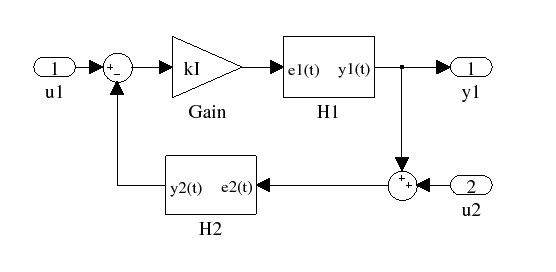
\includegraphics[width=0.95\columnwidth]{figures/fback_example}
    \caption{Block diagram interconnection example for feedback structure.}
    \label{fig:fback_example}
\end{figure}

Assume that the combined dynamic system $H:[u_1,u_2] \to
[y_1,y_2]$ depicted in Fig.~\ref{fig:fback_example} consists
of two dynamic systems $H_1:u_1 \to y_1$ and $H_2:u_2 \to y_2$ which
are respectively inside the sector $[a_1,b_1]$ and strictly inside the
sector $[0,1+\epsilon], \text{ for all } \epsilon > 0$.  Then $H$ is
bounded ($L^m_2$ stable for the continuous time case or $l^m_2$ stable
for the discrete time case) if:
\begin{equation*}
-\frac{1}{\max\{|a|,b\}} < k < -\frac{1}{a_1},\ \text{ if } a_1 < 0
\end{equation*}
\begin{equation*}
-\frac{1}{b} < k < \infty,\ \text{ otherwise.}
\end{equation*}

The extra output ports (numbered 2 and 3 in Fig. \ref{fig:fback_example}) in the diagram
will be covered later.  They represent points at which we attach signal monitors to perform
online assessment of the sector bounds.

\subsection{Digital Control Design Example}

Our design example controls a continuous-time system whose model represents a simplified 
version of a quadrotor UAV.  Fig. \ref{fig:quadrotor} depicts the basic
component architecture for the control design.  Our example excludes the
nonlinear rotational dynamics of the actual quadrotor for simplicity, but
retains the difficult stability characteristics. Fig. \ref{fig:qr_plant} shows
a Simulink model depicting the simplified dynamics.  For the fully detailed
quadrotor model and a complete discussion of the control design philosophy, see
\cite{quad:passcontrol}. The example model controls the stack of four
integrators (and motor lag model) using two nested PD control loops, including a nonlinear 
model element for actuator saturation in the outer loop.
%, as shown in the
%Simulink diagram shown in Fig. \ref{fig:qr_mdl}.  
The Plant block contains the
integrator models. The two control loops (inner and outer, as shown) are
implemented on separate processors, and the execution of the components is
controlled by a simple time-triggered virtual machine that releases tasks and
messages at pre-calculated time instants.

\begin{figure}[htb]
\centering
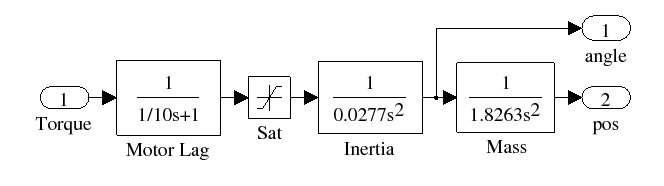
\includegraphics[width=\columnwidth]{figures/quadrotor_plant}
    \caption{Simplified quadrotor plant dynamics.  The rotational dynamics have
been removed to facilitate easier study of the behavior.  The full model
includes all of the dynamics.}
    \label{fig:qr_plant}
\end{figure}


\begin{figure*}[htb]
\centering
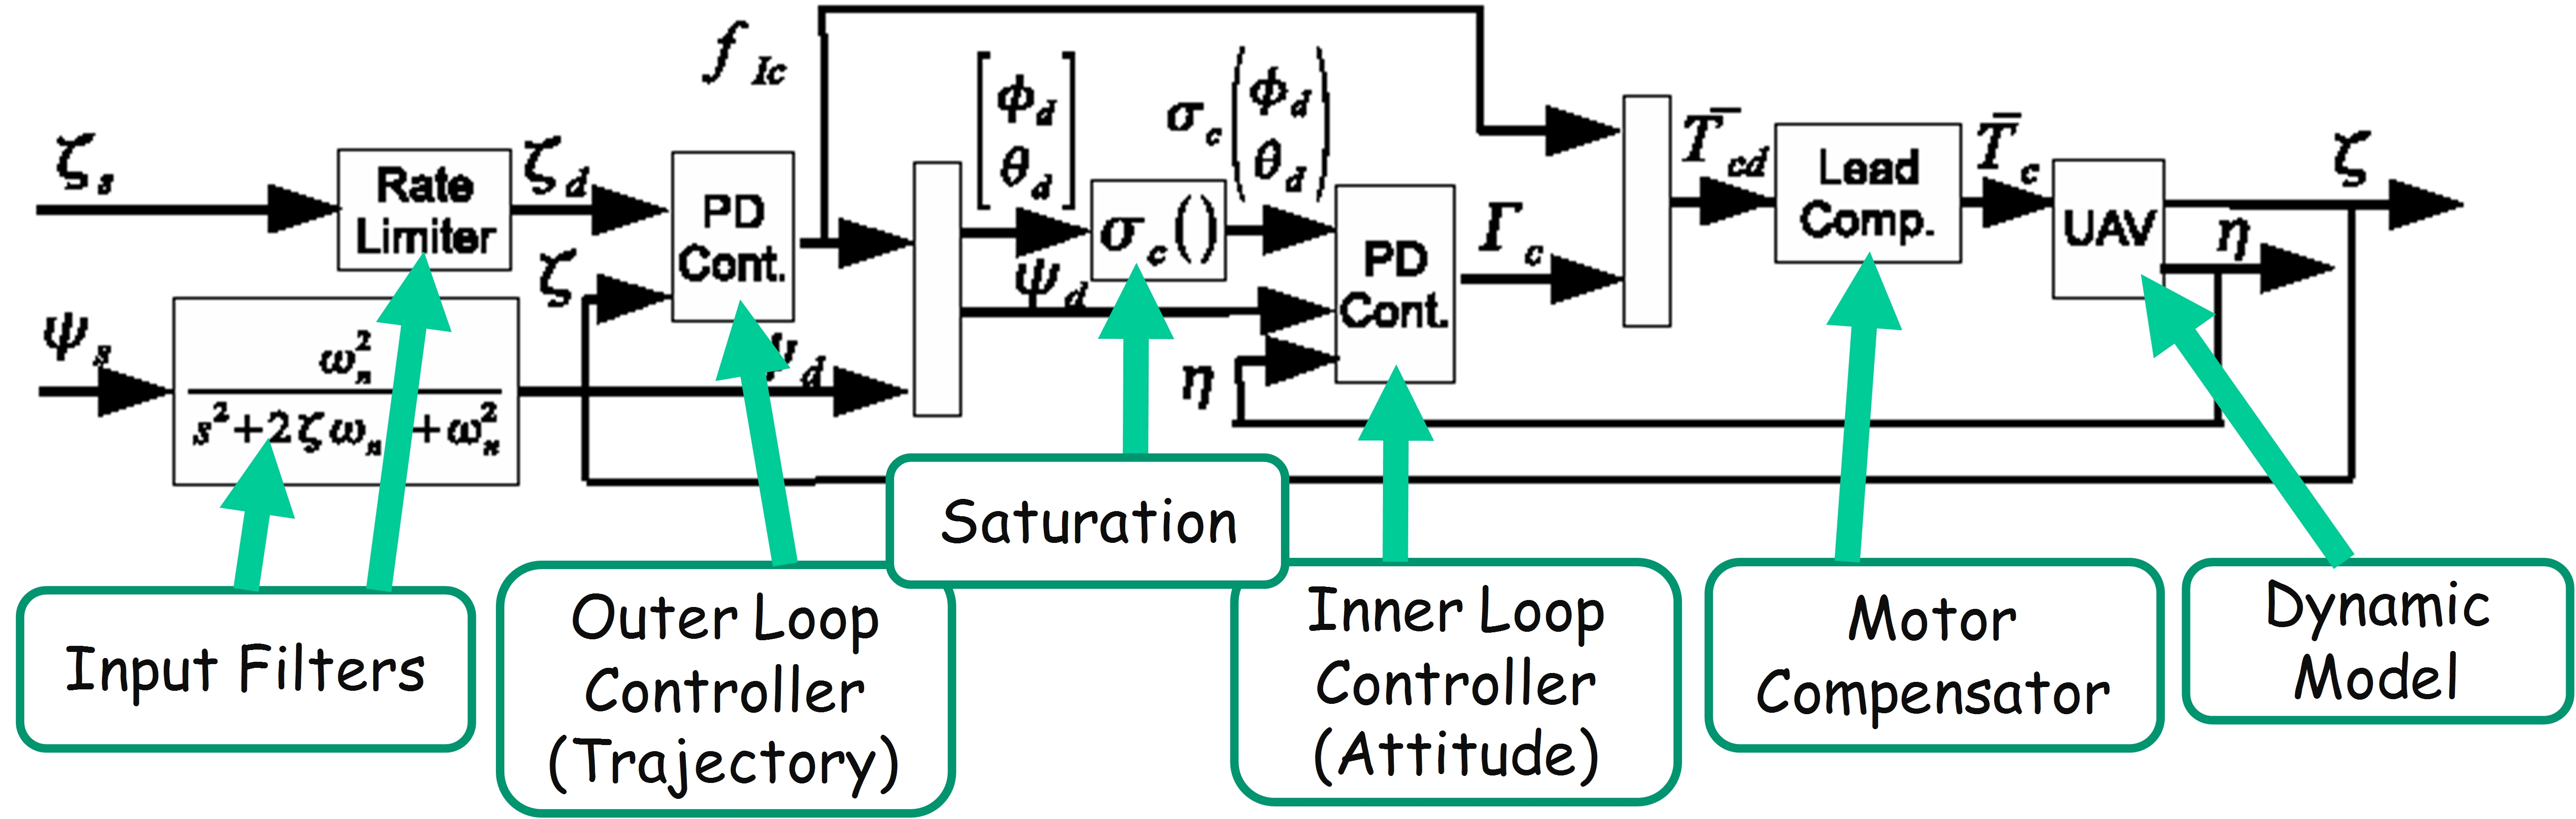
\includegraphics[width=1.75\columnwidth]{figures/quadrotor_arch}
    \caption{Basic architecture for the quadrotor control problem\cite{quad:passcontrol}.}
    \label{fig:quadrotor}
\end{figure*}


If the plant dynamics were passive, we would have considerable freedom in setting gains and
choosing control structures.  The combination of fast dynamics and new energy introduction
into the environment by the zero-order hold outputs means that each of the control loops must 
mitigate small amounts of ``active'' behavior.  The sector bound $a$ quantifies the 
energy-generating behavior of each control loop, but we still lose the flexibility of 
evaluating the design associatively while retaining the delay-insensitivity effects conferred
by passive structures. In our quadrotor system, we expect the bound $a$ to be small and 
negative and choose the gains appropriately.  

\begin{figure*}[htb]
\centering
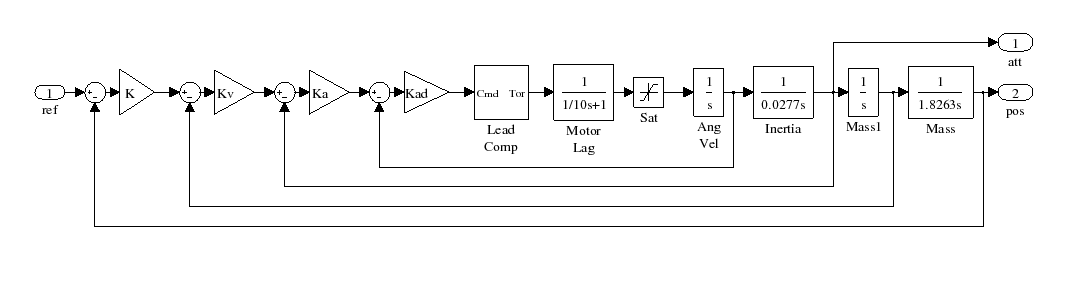
\includegraphics[width=2.2\columnwidth]{figures/quadrotor_loops}
    \caption{Conceptual nested loop structure of the controller.}
    \label{fig:quadrotor_loops}
\end{figure*}


This particular design must be evaluated from the innermost loop to the outermost loop in order
to make sense of the gain constraints. Fig. \ref{fig:quadrotor_loops} shows the nested loop
structure of the design.  The actual design and implementation are complicated by the 
physical architecture of the digital realization: 

\begin{enumerate}
 \item Sensors acquire digital attitude and position information, so velocities must be estimated.
 \item The controller components and velocity estimators are deployed to different processors in the 
digital implementation.  The two inner loop controllers, motor lead compensator, and angular velocity
estimator are deployed to an onboard controller with rich I/O capabilities.  The outer loop 
controllers and velocity estimator are deployed to a faster processor which also receives 
reference trajectory data.  Data messages are exchanged between the two processors using a 
time-triggered protocol.
 \item Motor thrust commands are issued periodically using a zero-order hold.  As discussed
previously, this introduces additional energy back into the environment.                                                          
\end{enumerate}










% 
% 
% \subsection{Passive Digital Control Using Sector Analysis}
% 
% Digital control systems present more of a challenge for the use of passive control
% techniques.  Digital control for physical systems with fast
% dynamics (such as a quadrotor helicopter) use a zero-order hold to convert control 
% values produced at discrete time instants into step functions held over a continuous
% interval of time.  For certain inputs and state trajectories, the hold process
% can introduce small amounts of new energy into the environment.  The sector
% bounds analysis proposed by Zames \cite{control:sectors1} can be used to assess
% the amount of ``active'' (energy-producing) behavior which we can expect from
% a design under nominal operating conditions. 
% 
% Using Zames\cite{control:sectors1}' formulation, the sector bounds for a
% control component are a real-valued interval $[a,b]$, where the endpoints come 
% from the expression in Eq. \ref{eq:sectors}.  Table \ref{tab:quantities} explains
% the terms.
% 
% 
% If we consider the instantaneous behavior of the system, a positive system gain 
% roughly corresponds to power dissipation, while a negative gain implies that
% the component is generating power.  Extending this idea to energy use up to
% a given time $T$, the same concepts apply\cite{pass:delasen}.  The sector technique 
% tries to bound any nonlinear elements in terms of their possible maximum and minimum gain, 
% and then uses composition rules to determine sector values for collections of elements.
% See Zames\cite{control:sectors1} for the discussion of composition rules, as we do not
% cover those here.
% 
% For linear (and some nonlinear) system models, sector bounds may be computed
% symbolically during system analysis.  Each component is assigned a real
% interval $([a,b] \, -\infty < a \leq b \leq \infty, \, b \geq 0 )$
% representing a range of possible input/output behaviors.  Components whose
% bounds fall in the interval $[0, \infty]$ are passive (and have some built-in notion
% of stability).   For our quadrotor system, we
% expect the bound $a$ to be small and negative, corresponding to the small
% amount of ``active'' behavior due to the hold effects. \cite{quad:passcontrol}
% shows a formula for selecting stabilizing linear feedback gains based on knowledge 
% of the value of $a$ ($ k < \frac{-1}{a} , \, a < 0$).  Here the gain $k$ is as shown
% in the loop diagram of Fig. \ref{fig:closedloop}.   In our online search any value of $b$
% up to infinity is acceptable.  As $b$ is also guaranteed to be positive, we do not 
% check for it.  We only search to estimate $a$ and ensure that it remains within the
% bounds prescribed by the selected control gains.

\subsection{Online Sector Analysis}

% \begin{figure}[tb]
% \centering
% 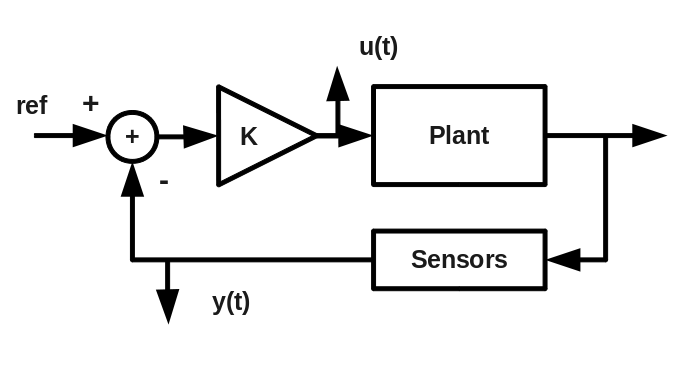
\includegraphics[width=0.8\columnwidth]{figures/control_loop.png}
%     \caption{Closed feedback control loop. $K$ is the controller gain, $u(t)$ is the input to the sector search for this loop, and $y(t)$ is the output.}
%     \label{fig:closedloop}
% \end{figure}

\begin{figure}[tb]
\centering
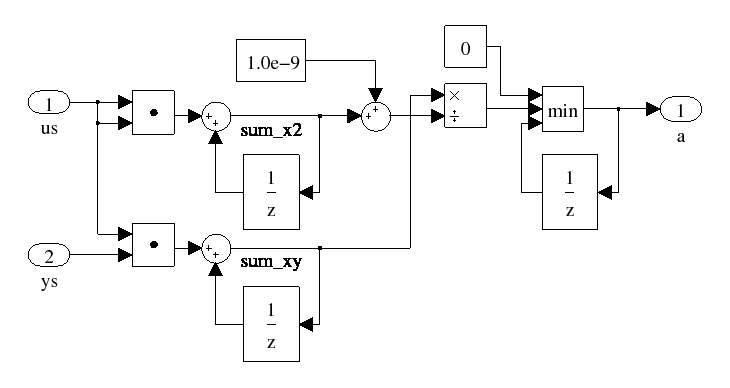
\includegraphics[width=\columnwidth]{figures/srch_block}
    \caption{Simulink implementation of the online sector analysis algorithm.}
    \label{fig:sectorsearch}
\end{figure}

Fig. \ref{fig:sectorsearch} shows the structure of an online sector calculator in Simulink.  We 
refer to its implementation as the (possibly misnamed) online sector search or the sector 
analyzer -- it is included with deployed digital controller code to assess stability by monitoring 
the estimated sector values. The C source was generated using Real-Time Workshop.  The block 
input $x$ corresponds to the input variables to be monitored, and $y$ to the output
variables to be monitored.  The sector analyzer operates by calculating the accumulated 
input energy and dissipation terms for each sample, computing their ratio (the sector 
value so far), and maintaining the minimum.  The calculated sector bound value decreases 
monotonically, and we rely on the calculated bound achieving a steady-state value (settling to 
a constant in the limit) for a particular input.  The minimimum over all realizable inputs is 
the sector bound for the system. The ``search'' concept refers to the 
idea that we explore these bounds over a range of inputs and controller parameters 
to find the worst-case bound to use during operation.  In online 
operation the sector calculation is not a ``search'' as much as a validation of behavior 
with respect to our analytic and simulated sector values.  The name ``sector search'' has
stuck, though.

Empirical verification of the sector bounds does not provide a necessary condition to verify
stability for the implementation, but it is sufficient. If sectors are estimated conservatively, 
then measurements which exceed the bounds are significant.  This indicates 
that the selected control gains may not have been adequate to stabilize the system with the 
platform delay and quantization effects included in the closed-loop controller.  In our case an 
input which drives the maximum output slew rate should yield the largest active sector bound
value.

\newpage

\subsection{Limitations}

The current implementation of the online sector analysis has a few limitations:

\begin{itemize}
 \item The sector calculation implementation is an approximation, the error of which may be
aggravated by our $\epsilon$ term which is used to prevent divide-by-zero  
(in Fig. \ref{fig:sectorsearch}, for example, $\epsilon$ is $1.0e-9$).  In this form the 
estimated sector bounds could be smaller than the actual bound.  In that case the online 
search could fail to detect small trajectory deviations that might indicate instability.  
In practice the difference is small or negligible, and the sector analyzer is sensitive enough 
to capture platform effects.
 \item The sector calculation in its current form requires high precision.  We use 
double-precision floating point, as even single-precision calculations introduced 
instability in the sector calculation.  This may be a significant obstacle for deployments
to small embedded controllers that lack floating-point hardware.  For the experiments on actual
hardware we were required to export much of the sampled data out of the control processors in order 
to perform the sector search with sufficient precision, despite the availability of sufficient 
runtime to do the calculations on the controllers.
\end{itemize}

Both of these deficiencies could be remedied by a more careful design of the search
implementation.  In particular, a good fixed-point implementation would be very useful
for deployment to microprocessors that lack floating point capabilities.  Another approach
which avoids introducing computational overhead is to use external signal measurement 
devices and perform the sector analysis externally using another computer. This could be 
done using a digital scope for electric signals, a JTAG debugger to get digitally stored 
values, or a logic probe.
